\subsection{Chainer-MNIST}
%
The intention of this section is to evaluate the performance of a handwritten digit recognition application that uses PyMic to perform parts of computation on Intel Xeon Phi coprocessor. Our experimental evaluation focuses on two aspects. The first one is the different between CPU and coprocessor computing capabilities, the other one is the potential of using PyMic in machine learning and deep learning applications.
\subsubsection{Chainer-numpy:}
%
Chainer is a well known framework for Artificial Neural Network(ANN). One of its advantages is flexibility, which enable its users to create complex architectures simply and intuitively. Similar to TensorFlow[*], Caffe[*] or Theano[*], Chainer uses back-propagation algorithm [*] for training data and adjusting network's parameters. However, by using "Define-by-Run" scheme,  the network is defined on-the-fly while running actual forward computation, it make an network created by Chainer become easier to debug than other frameworks. Therefore, an application written by Chainer integrated Pymic have a faster development time.
%

\subsubsection{Experimental Setup:}
%

Our experiments was performed on a combination of CPU Intel Xeon E5 and Intel Xeon Phi 7120P coprocessor. The technical specifications of our system are described in table [*] . The framework was compiled for coprocessor using Intel compiler [*]version as well as OpenMP parallel programming API implementation by Intel  and MKL [*]version. All measurements were carried out multiple times and averaged to eliminate variances in the resulting measurements.
%
\begin{table}[]
\centering
\caption{Technical characteristic of System}
\begin{tabular}{|c|c|c|}
\hline
\textbf{Codename} 	& \textbf{CPU} 	& \textbf{Coprocessor} \\ \hline
\textbf{Model} & Intel Xeon E5-2680V3  & Intel Xeon Phi 7120P \\
\textbf{Microarchitecture} & Sandy Bridge EP & Intel Many Integrated Core \\
\textbf{Clock frequency} & 2.50/3.30 GHz & 1.24/1.33 GHz \\
\textbf{Memory Size} & 512 GB & 16 GB \\
\textbf{Cache} & 30.0 MB SmartCache & 30.5 MB L2 \\
\textbf{Max Memory Bandwidth} & 68 GB/s & 352 GB/s\\
\textbf{Core/Threads} & 12/24 & 61/244 \\
\hline
\end{tabular} 
\end{table}


We evaluated our approach using the MNIST [*] dataset of handwritten digits including training set of 60,000 examples,  and 10,000 test images, each image contains 28x28 pixel grey levels. The testing ANNs architecture have 1000, 1500, 2000, 2500 ... 5500 unit, each unit represents a node in the network's hidden layer. In order to simply the performance evaluation process, we just modify the ANNs with one hidden layer, that mean our ANNs have only 3 layers which are input, output and hidden. Detailed information of the ANNs used in our evaluation are shown in Table[*].
%
\begin{table}[]
\centering
\caption{ANN architecture}
\begin{tabular}{|c|c|}
\hline
\multicolumn{2}{|c|}{\textbf{ANN Configuration}}\\ \hline
\textbf{Layer} 	& 3 \\
\textbf{Batch Size} & 60000 \\
\textbf{Connetion Function} & Linear  \\
\textbf{Activation Function} & Relu  \\
\textbf{Loss Function} & Softmax Cross Entropy \\
\textbf{Gradient Method} &  Stochastic gradient descent \\
\hline
\end{tabular} 
\end{table}
\subsubsection{Result:}
%
We intend to perform entire evaluation on docker in order to easily customize the constrains of system resources. A simple experiment was conducted to ensure that the execution of the ANNs in docker is similar to physical machine and we obtained the expected result. Thereafter, we started to evaluate the performance  application, written by two version of Chainer, one is original version and the other is PyMic integrated version, called Chainer-XP , to execute on Intel Xeon Phi coprocessor.
\begin{figure}[]
\centering

\includegraphics[scale=0.6]{img/a.pdf}
\caption{Chainer-XP 1 core and full core}
\end{figure}

Results presented for Chainer-XP in Figure [*] show that all experiments of our ANNs training corresponding to number of Units: 1000, 2000, 3000, 4000 and 5000, were executed in roughly equal time periods without being influenced by the number of CPU cores. That also means most of the computational function have been offloaded into Inter Xeon Phi coprocessor. Moreover, it can be seen that the data communication occupies most of execution time of training process, overhead is caused by the synchronization between CPU(host) and coprocessor(device) during the calculation. Overall, PyMic are an potential framework which support its user run ANNs entirely on Intel Xeon Phi. However, the synchronization occupies a prominent role throughout the training process, if it is not tightly controlled, the performance can be devastatingly reduced.


In this experiment, we intend to evaluate PyMic's computational capabilities in Intel Xeon Phi. The first ANN (ANN-1) written by original Chainer was executed on a docker that used full core of a CPU Intel Xeon E5, and the other ANN(ANN-2) written by Chainer-XP on a docker used only one core combined with Intel Xeon Phi coprocessor. In detail, both ANNs contains three layers and 1000 units in hidden layer, the networks configuration details are described in the Table [*]. Then we measured thoroughly the execution time of all function during training process and found out that with the second ANN calculation time on coprocessor occupies just approximately 29.2\% total run time. More specifically, with a mentioned ANN, the calculation is mainly execute in \textit{dot} function, about 90.2\% of all time execution as it is called three times each training.
\begin{figure}[]
\centering
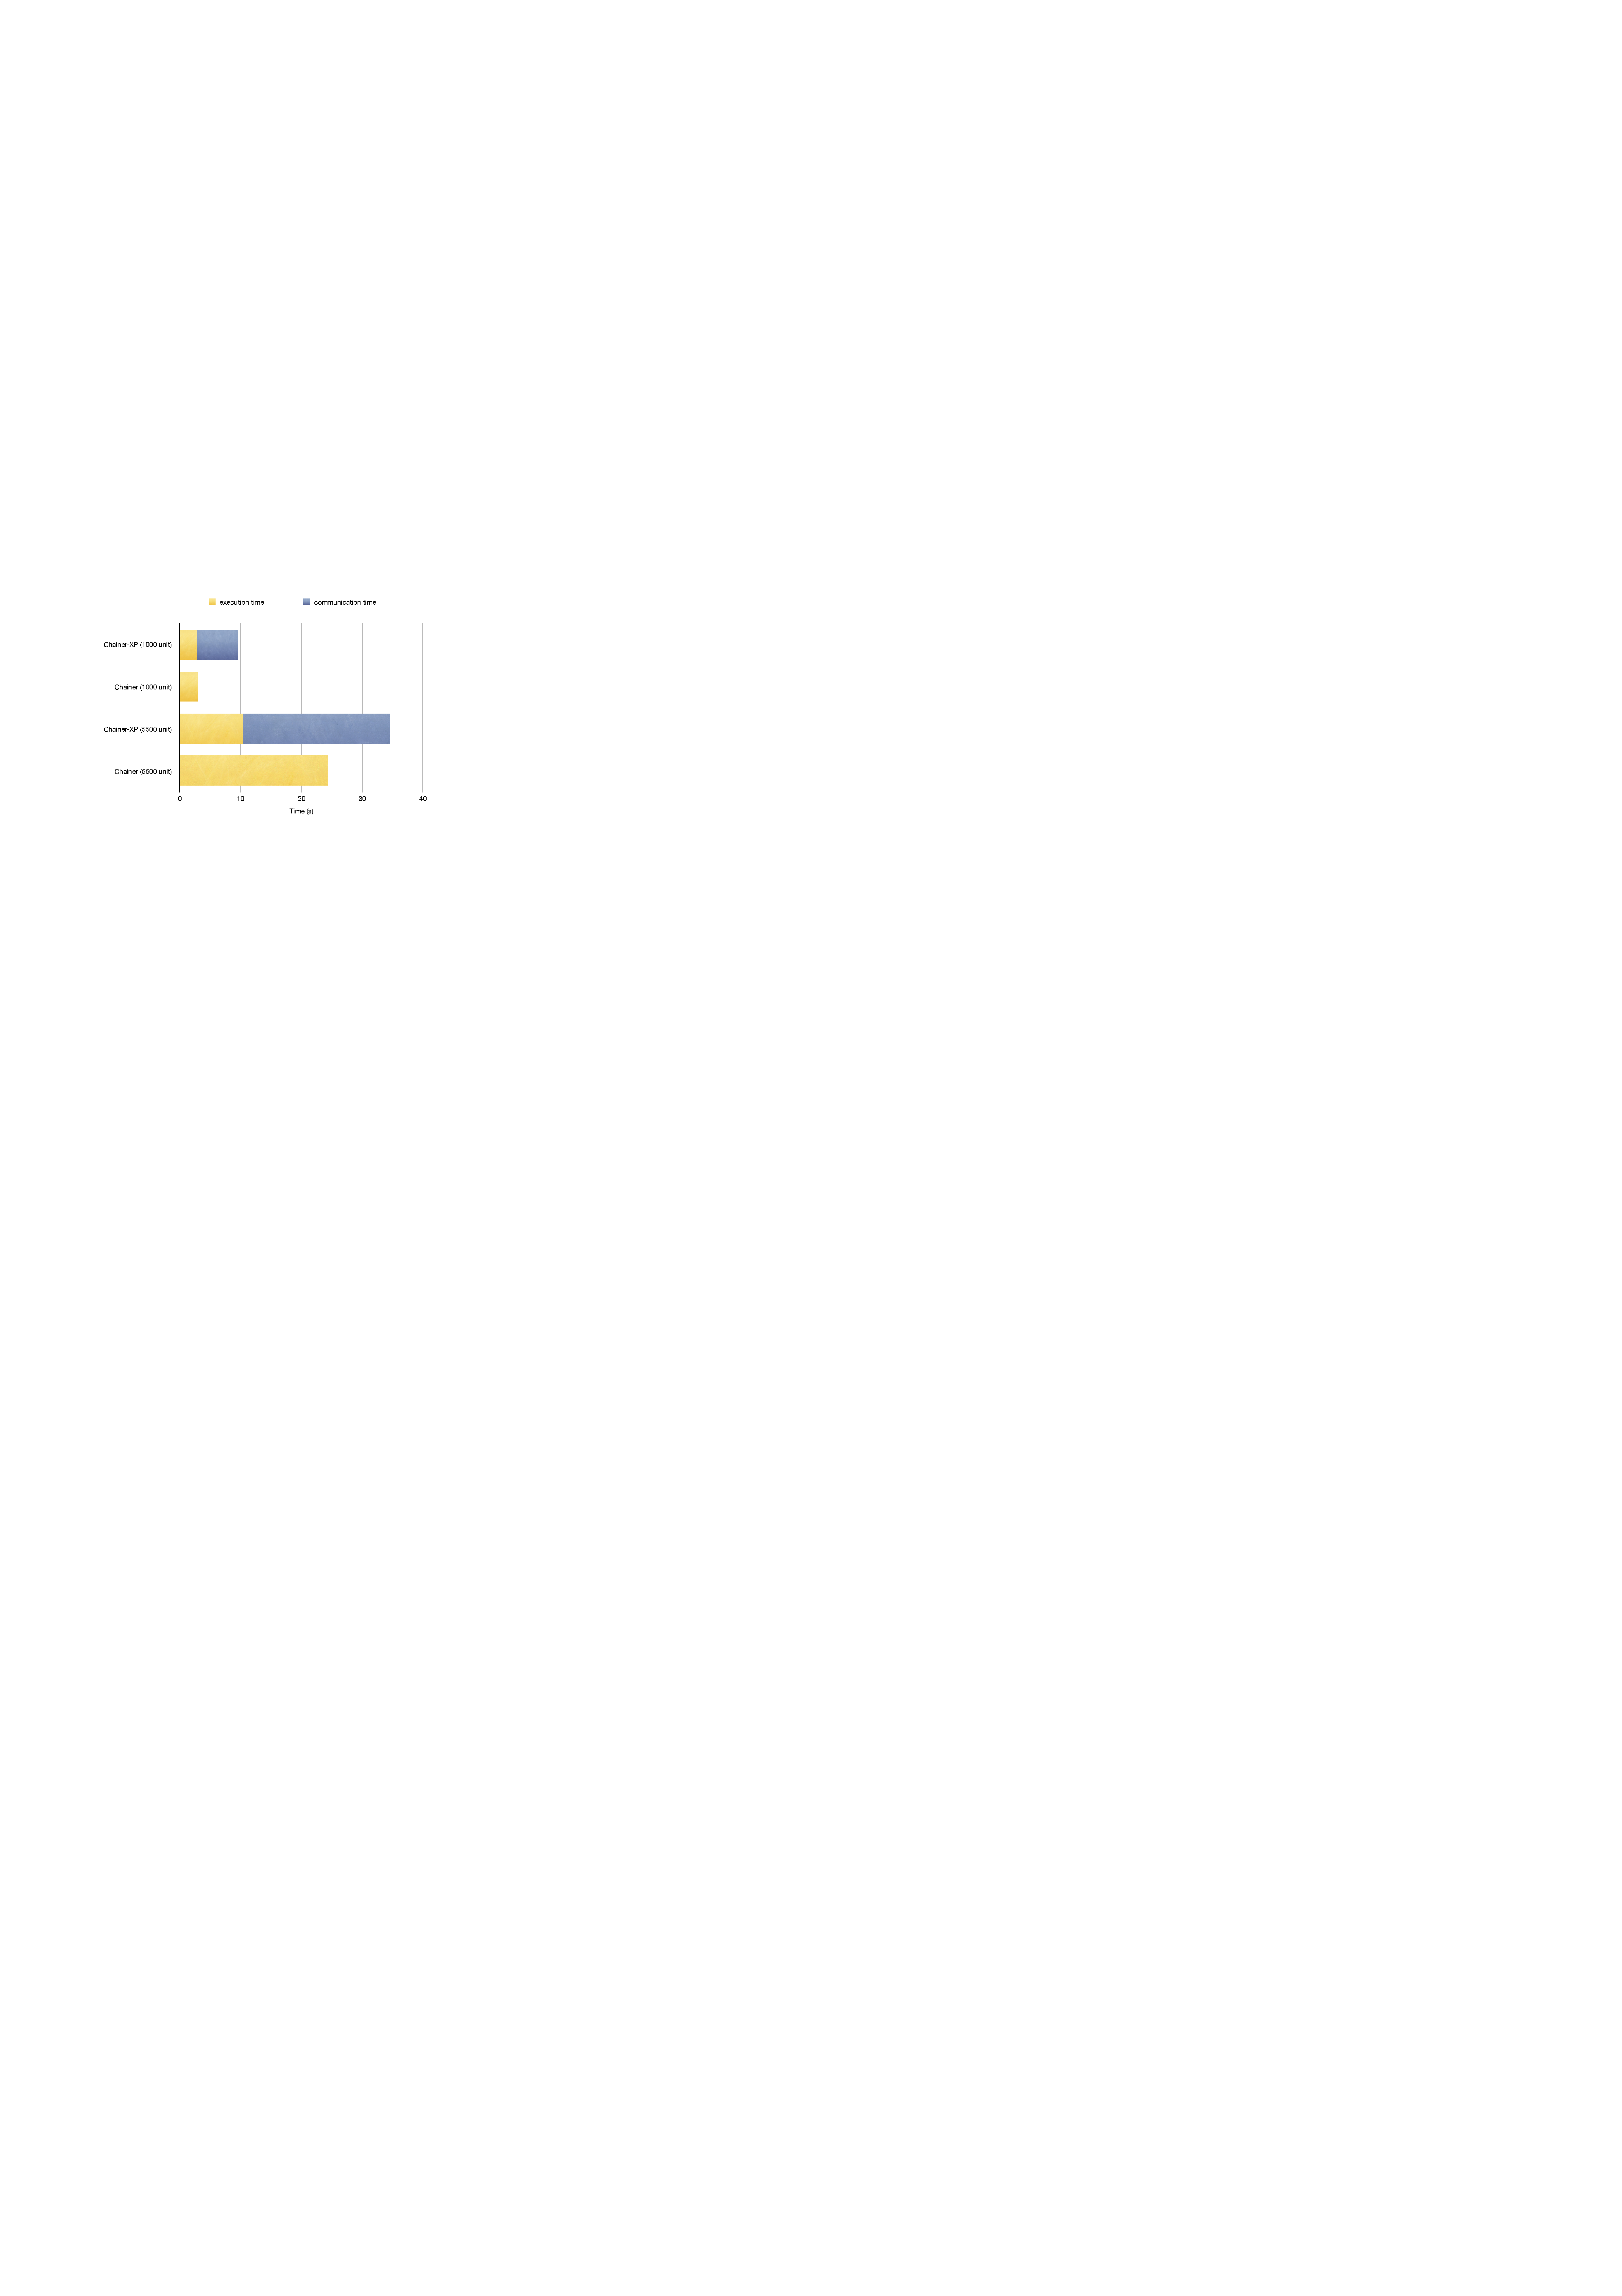
\includegraphics[scale=0.5]{img/b.pdf}
\caption{Chainer-XP 1 core and 12 core}
\end{figure}

The biggest matrix size that the \textit{dot} function must perform during the execution of the above network is [784,60000] x [60000,1000], which corresponding to 70.8\% total run time were use to synchronize data between host and device. Although the purely  computing time on the coprocessor was approximately 1.93 times faster, the total training time was about 1.78 times slower than the full CPU. The reason for this drop in performance is data was transmitted between hosts and devices repeatedly leading to overlap and redundancy. However, the caused of this result is the PyMic integration into Chainer has not been optimized, so that the we can significantly improve the result as PyMic provides objects and functions that strictly support allocate and deallocate memory on Intel Xeon Phi coprocessor. In other words, we must fully understand how Chainer organizes the data so that we can reduce the communication between host and device and increase the performance of training process. As mentioned, in this paper we just focus on the computing capabilities so in the rest of the experiment, the number of units was raised to 5500 with the aim of increasing the size of the largest matrix to [784,60000] x [60000,5500]. The observed result show that the ratio between execution time on coprocessor and total training time was almost unchanged at about 30\%. In addition, when the size of one of the two DOT operands expanded 5.5 times, the computation time on the Intel Xeon Phi increased only 3.8 times, while the CPU grown up to 7.8 times, and total training time achieved 1.2 times faster than CPU. Thus, with several medium configuration CPUs, there is the possibility that we can speed up with Intel Xeon Phi for large-scale computing in ANNs.
\begin{figure}[]
\centering
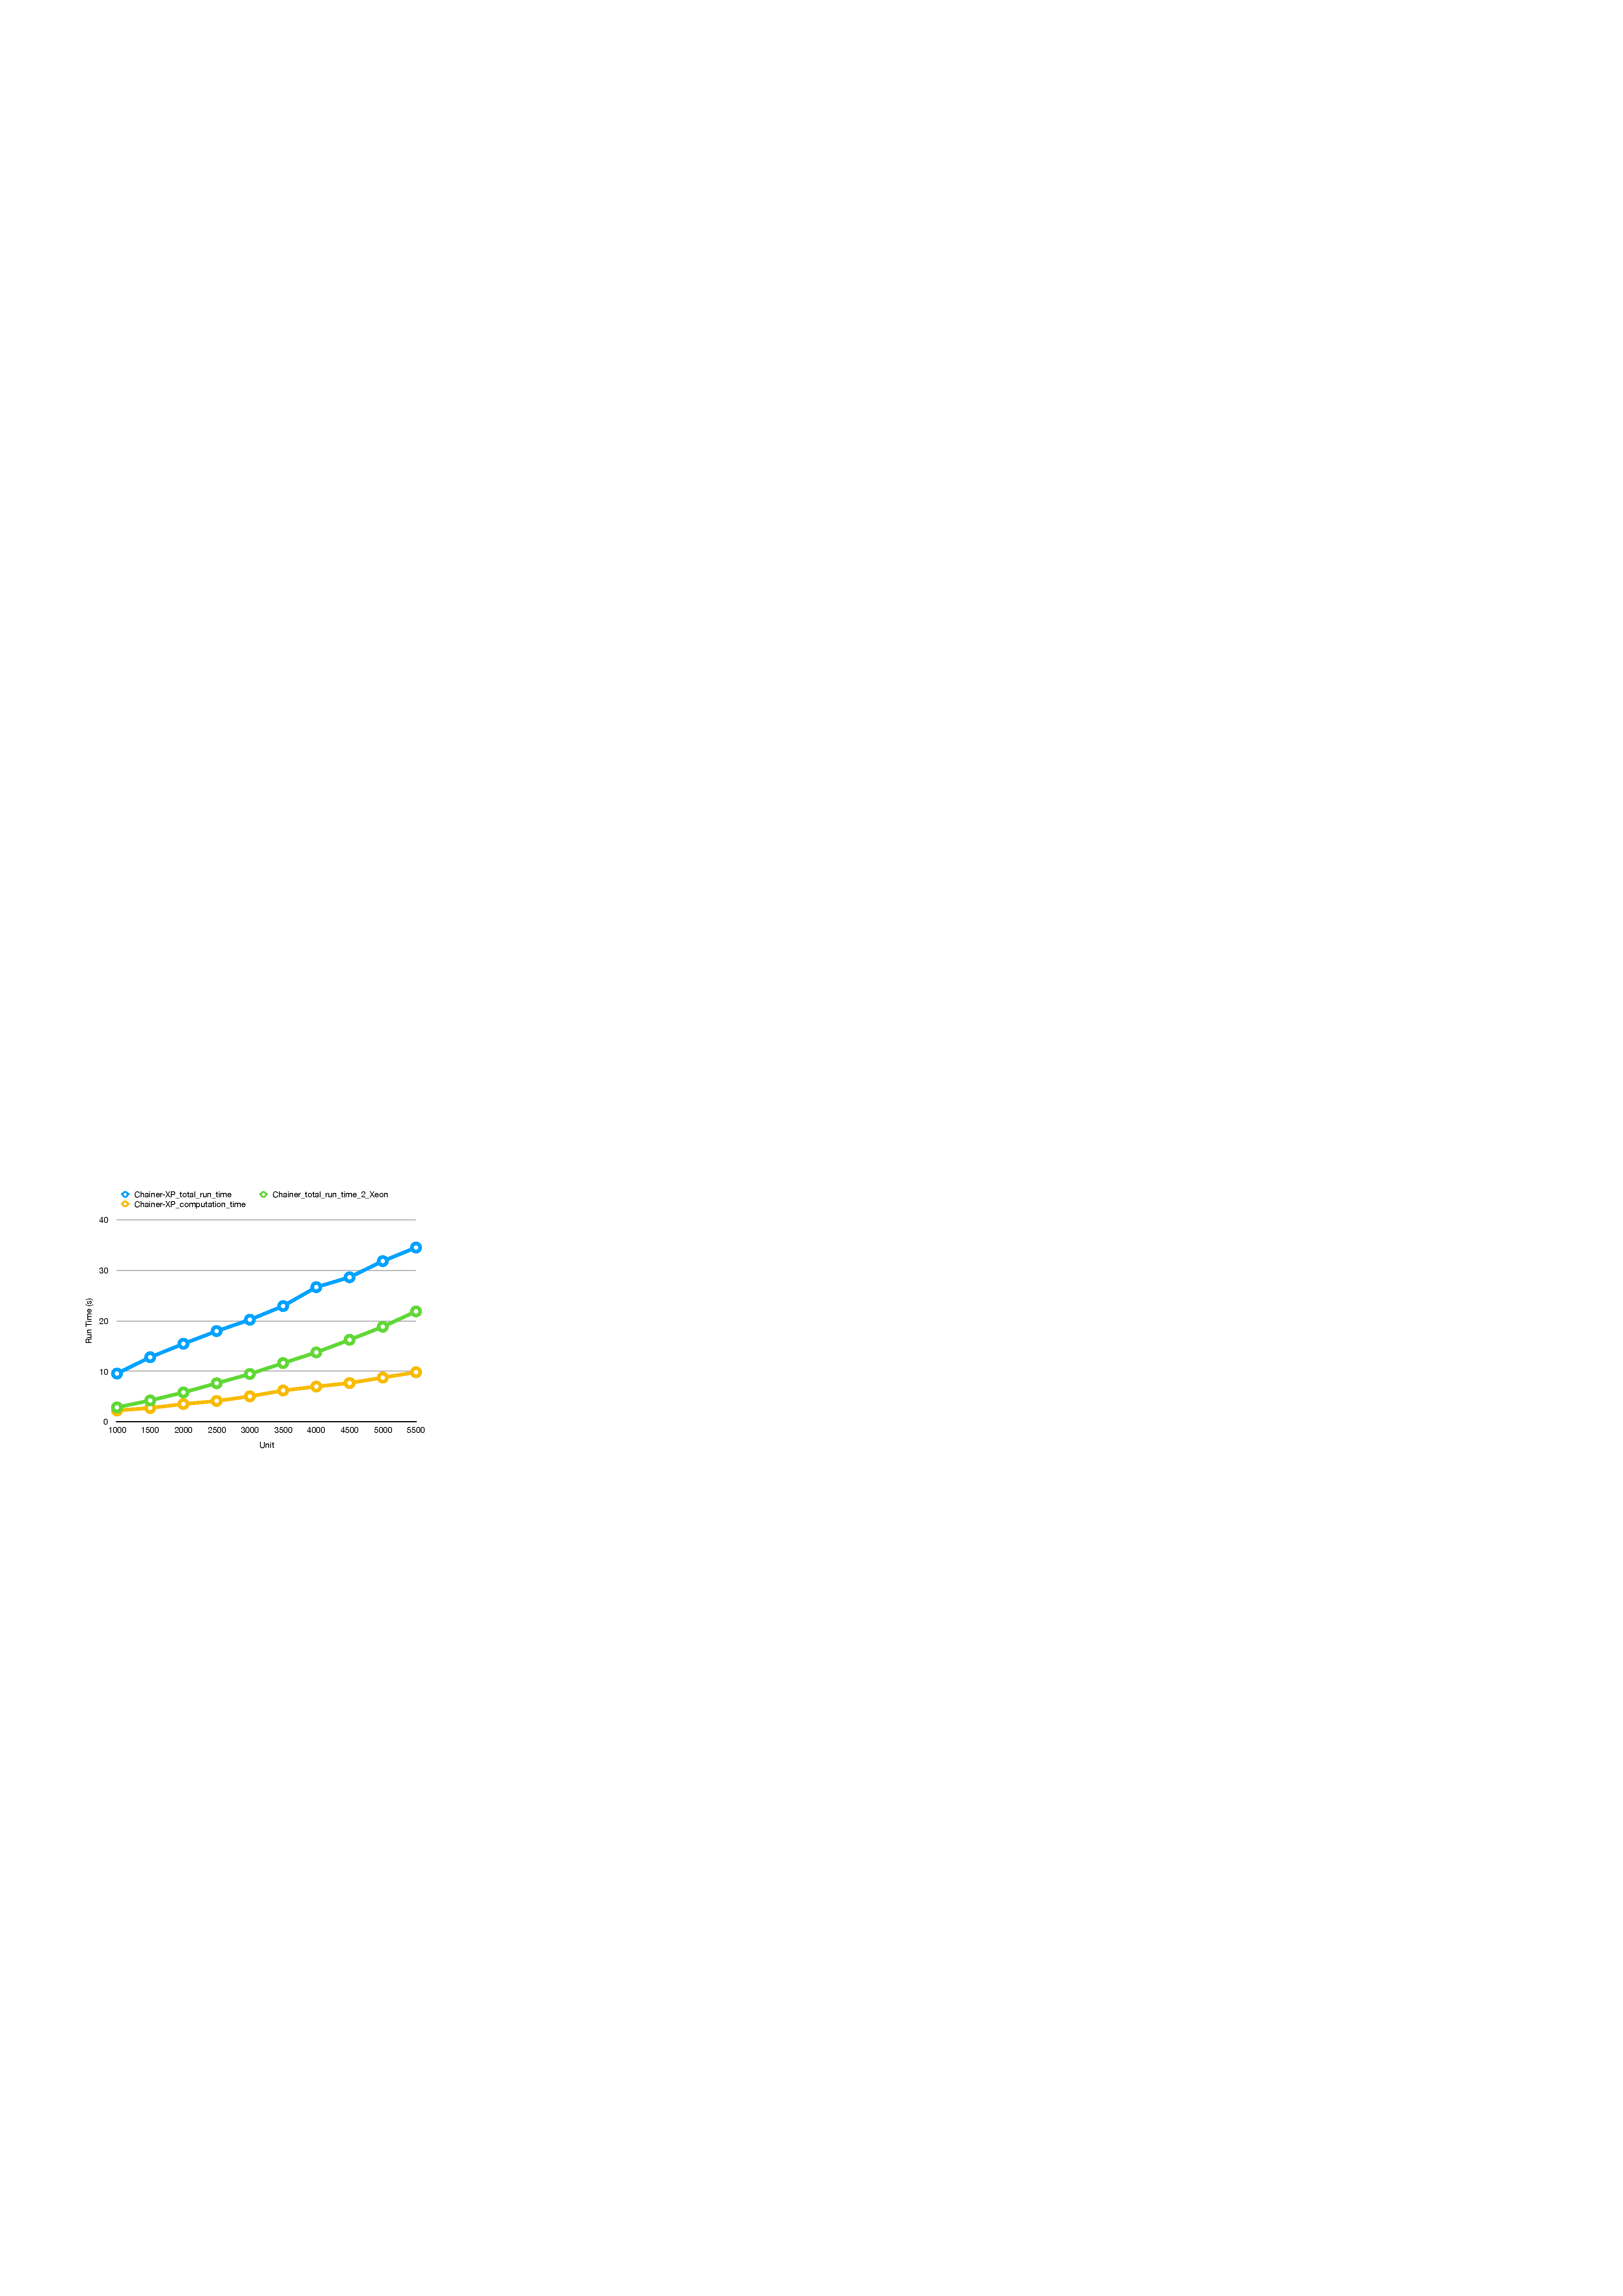
\includegraphics[scale=0.6]{img/c.pdf}
\caption{Chainer-XP vs Chainer}
\end{figure}

The comparison between two version of Chainer is illustrated in Figure [*]. In order to obtain this experience, The ANN-1 was executed entirely on CPU with a docker containing dual-processor Intel Xeon E5, which has computing capability approximately 960 GFLOP/s, while the theoretical peak performance of an Xeon Phi coprocessor is 1 TFLOP/s [*] in double precision. Although they almost have the similar processing power, execution time of an ANN integrated PyMic  is getting faster and faster than this ANN which run in CPU. Hence, It can be seen that Pymic has used the Xeon Phi SIMD mechanism, as well as Vectorization technique of Intel Xeon Phi quite effectively in calculating sequential elements.
